\chapter{AccessibleEPUB Editor}
\label{ch:AccessibleEPUB Editor}

In this section the Accessible EPUB editor will be presented with the requirements it should have. After that there will be an evaluation where the various problems and issues faced during the development will be explained and how they were solved.

\section{Existing EPUB editors}
\label{ch:exEPUB}
There are a number of different ways to create EPUB documents \cite{EPUBprograms}. Adobe InDesign\footnote{https://www.adobe.com/products/indesign.html} is one way and is suitable for publishers, but it has no built-in MathML support and it is a commercial program that is unaffordable to most user groups. LibreOffice in its latest version 6.0 is able to export Writer documents to EPUB, too. This and perhaps Microsoft Word (with installed EPUB macros) are maybe the easiest options to create an EPUB document. Nevertheless, these versions have to be edited after export in special EPUB editors to meet proper accessibility levels, like adding alternative texts for images or LaTeX source code alternatives for mathematical formulas.
Some EPUB editors are pure WYSIWYG editors (What You See Is What You Get), but important functions such as mathematical equations and semantic information are usually missing. EPUB editors where the program code has to be edited are limited to individuals with programming experience. Sigil \cite{Sigil}, for example, is an open source WYSIWYG EPUB editor with many features, but important features such as text alternatives for images can only be added manually with coding.
Most editors are not able to produce the kind of universal accessible document desired out of the box, nor are they accessible to visually impaired or blind people. 

\section{Requirements}

There are a variety of requirements which have to be fulfilled by a suitable editor. Most importantly, it has to be easily usable and not require any programming knowledge to use, except LaTeX code for equations. Currently no other EPUB editor allows users to insert equations without them explicitly programming it in. The technology required for EPUB documents must be done behind the scenes and the user must not be exposed to it. 

\section{Programming language}

The first question was in which programming language the editor should be implemented in. C\# and Java were picked as the two main options, as both of them are object oriented and natively support graphical user interfaces (GUI). Furthermore, both support the ability to make the programs themselves accessible, e.g. for blind users. C\# has several accessibility properties, like AccessibilityDescription and AccessibilityName, which are passed to the screen reader. Java uses the Java Accessibility Bridge which makes it accessible to screen readers. Java is platform independent, and while C\# programs can run on Mac OS and Linux, it relies heavily on Windows and its features. However, Java is not already installed on any operating system, while C\# programs can run on Windows machine with only .NET as prerequisite. The target .NET version of the editor is contained in Windows 10. Therefore the editor was programmed in C\#, as the users were predominantly Windows users and don't have to install any prerequisites.

\section{Features}

\subsection{Main window with editor and preview}

The main window is the entry point of the program, shown in both figures \ref{fig:formJs} and \ref{fig:formCss}. At first it has a splash screen in the central panel which then shows an editor and a web browser. The content typed into the editor is converted into HTML code which is then displayed in the browser and updated automatically. The web browser can display the content in each of the three versions mentioned in chapter \ref{ch:EPUB Document Standard}. The toolbars at the top contain standard editor tools, such as making the text bold. It also contains some specialized tools, specific to this program. Some of them allow the user to add HTML elements like mathematics, tables or images. Other specialized tools allow the user to show and hide certain panels in the main window, such as the preview on the right hand side. 

\subsubsection{Editor}

\begin{figure}
	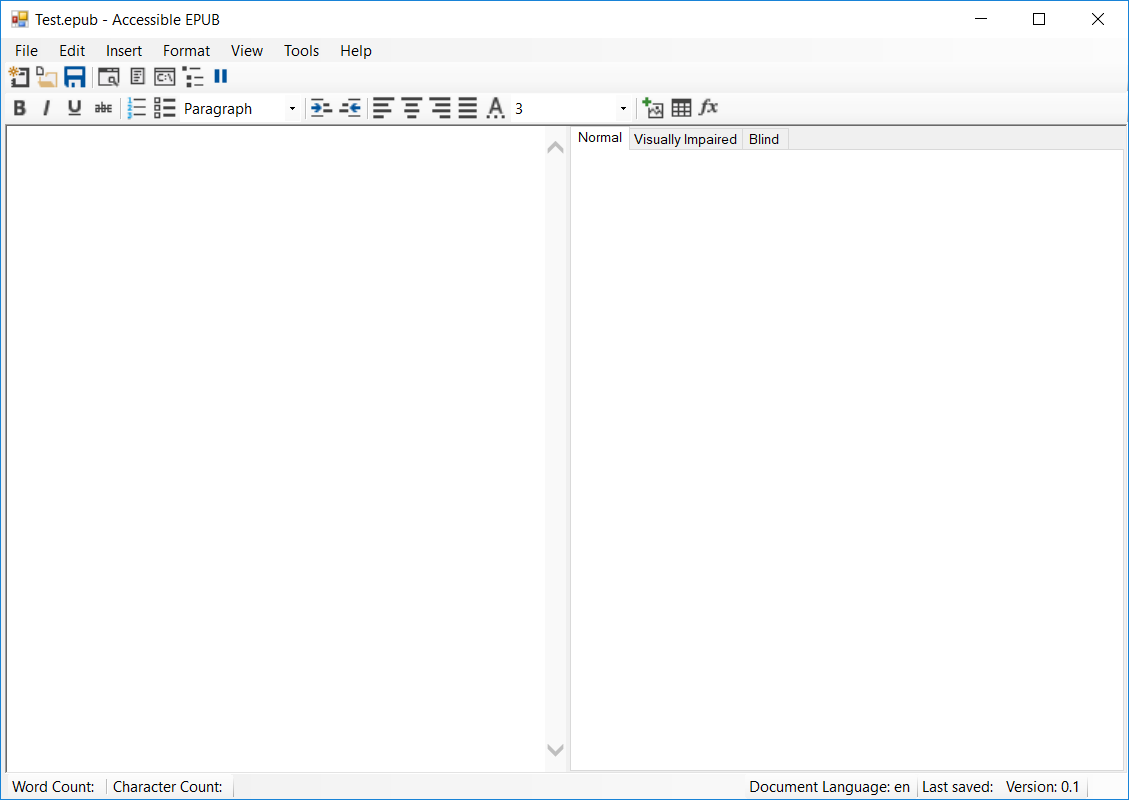
\includegraphics[width=\linewidth]{figures/formJs.png}	
	\caption{Main window with editor and JavaScript switching preview}
	\label{fig:formJs}
\end{figure}

The main window required the most programming and therefore also had its fair share of problems. The first issue was regarding the editor on the left hand side in figure \ref{fig:formJs}. At first a WYSIWYG editor was not intended, as it hides semantic information about the EPUB. The initial approach involved editing semantic information of XHTML elements, like images, and changing things like the \lstinline|src| for source, \lstinline|alt| for alternative text, etc. This was still in the early, rough stages and the approach seemed too complicated, so the WYSIWYG editor was chosen instead. 

The second issue was how to implement the WYSIWYG editor. Programming it from scratch would not be possible in the time allocated to a bachelor thesis, as it would involve creating a browser engine. Fortunately, the inbuilt browser in C\#, WebBrowser, allows editing with just a few lines of code. The WebBrowser control is based on Internet Explorer and displays web pages like it. It uses Internet Explorer version 6 as default, which does not display certain CSS properties such as \lstinline|max-width|. It adjusts images to fit to the size of the screen and it is vital for Accessible EPUB. To fix this issue, some code has to be run when the form has loaded which determines the Internet Explorer version on the computer and loads the newest one to the editor. After this SVGs and the CSS properties worked as desired. 

A major issue with the editor is that content written in it is converted to HTML, while EPUB requires XHTML. While there aren't major differences, there are some small ones such as independent tags like \lstinline|<br>| have to be self closing and written as \lstinline|<br/>| in XHTML. If this is not done the EPUB reader will specify an error. Therefore a tool has to convert the HTML code to XHTML. There are several packages available, one of them being HtmlAgilityPack\footnote{http://html-agility-pack.net/}. It can convert HTML to XHTML and also correct HTML parsing errors such as not closed tags. HtmlAgilityPack delivered good results at first. However, there soon was an error. Many mathematical signs, such as the sign "$\wedge$", were displayed as question marks. This meant that HtmlAgilityPack could not be used. 

Another available package was TidyManaged\footnote{https://github.com/markbeaton/TidyManaged}, but it did not convert the code properly to XHTML. The third attempt used SgmlReader\footnote{https://github.com/lovettchris/SgmlReader}, which converts SGML content, like HTML, to XML content, like XHTML. It successfully parsed the HTML and was able to convert mathematical signs properly. It did not create a XML declaration at the top of the document, but this was simpler to solve. A standard XML declaration was just added to the document and the new XHTML document was properly rendered by the browser.


\begin{figure}
	\begin{center}
		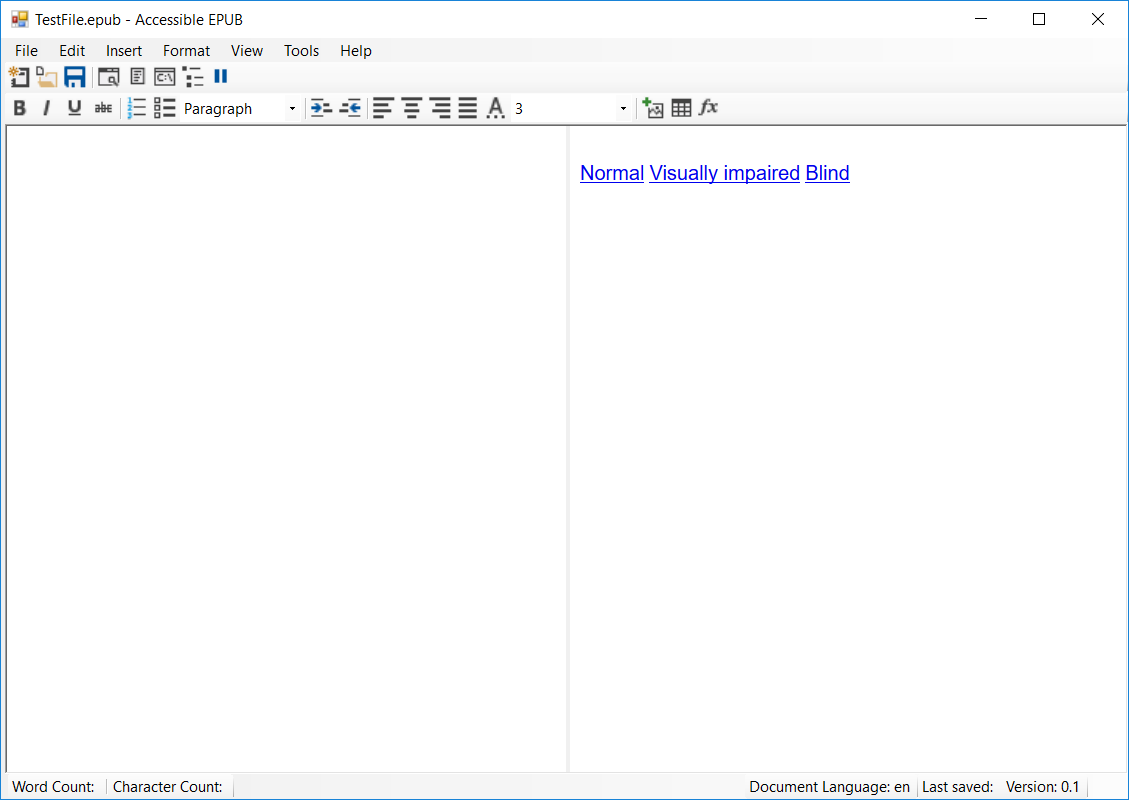
\includegraphics[width=\linewidth]{figures/formCss.png}	
		\caption{Main window with HTML editor and CSS switching preview}
		\label{fig:formCss}
	\end{center}
\end{figure}

\subsubsection{Preview browser}

On the right hand size of the main window is the preview browser. It should display the XHTML page in each of three versions (normal, visually impaired, blind). Since the HTML editor uses the WebBrowser control, it would have been easiest to use it on the right side too. However, Internet Explorer is unable to display MathML. Instead of showing the quadratic equation, as shown in figure \ref{fig:quadEquaPng}, it showed figure \ref{fig:IEmathml}. As a result, another preview solution had to be found. Only two browsers are able to properly show MathML, Mozilla Firefox and Safari by Apple. The Firefox engine, Gecko, was chosen as it is open source and had a C\# browser package. After inserting an instance of a \lstinline|GeckoWebBrowser| in the window MathML was displayed properly.

\begin{figure}
	\begin{center}
		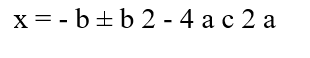
\includegraphics[width=\linewidth/2]{figures/IEmathml.png}	
		\caption{MathML depiction of the quadratic equation in Internet Explorer}
		\label{fig:IEmathml}
	\end{center}
\end{figure}

As seen in figures \ref{fig:formJs} and \ref{fig:formCss}, there is a small difference between the user interface of the JavaScript and CSS versions. The CSS version only uses one browser tab as preview, while the JavaScript version uses three. This is mentioned in chapter \ref{ch:EPUB Document Standard} and is due to the JavaScript version having a separate file named \lstinline|VersionChanger.xhtml|, which handles switching versions. In the CSS version the whole content is in one XHTML file. Consequently, the CSS version is very easy to show in the preview. Only the three links shown in figure \ref{fig:css_switch} have to be added to HTML editor content and file is done.

This is much more complicated in the JavaScript version, since the default display style will always be shown. The CSS of the blind and visually impaired version had to be changed. The initial attempt to solve this problem was done by changing the CSS of each browser in a tab and accessing the CSS properties, \lstinline|GeckoStyleSheet|, of the preview browser. Unfortunately, even after changing the \lstinline|GeckoStyleSheet| of a document, it still displayed the default one. An alternative approach consisted of accessing the head (\lstinline|<head>|) of the XHTML document and inserting the CSS there, but this too did not work. These two methods were preferable as they do not have significant input and output (IO) operations. Unfortunately, even slightly altered methods of the two did not work properly. As such an IO intensive approach had to be taken. The XHTML file with the content, \lstinline|Content.xhtml|, had to be copied to two new files, \lstinline|BliContent.xhtml| and \lstinline|ImpContent.xhtml| for the blind and visually impaired version, respectively. Then the single line linking the style in the XHTML head was replaced with one linking the corresponding CSS. 
Both files are removed before saving the EPUB and then created again. Thus there is additional overhead, but it was the only method which succeeded.

An important feature of Accessible EPUB is updating the preview after a change in the HTML editor. Originally this was done only after saving the document to reduce overhead. However, this does fulfill the requirement of live updating the preview. A timer was created in the program which updates it every second. This produced substantial overhead, slowing the program down when large images are added. Changing the timer to five seconds addressed this issue. 

After the preview is refreshed, it always get scrolled to the top. While this is not an issue in short documents, in long documents it is irritating to the user. The first approach involved saving the X axis and Y axis scroll bars' position, but it wasn't possible to get their values properly. A pseudo fix was designed instead which pauses the refresh after the user presses the pause button in the toolbar. This does not solve the issue, but it makes it less irritating to the user.

A feature which was also added was the ability to change the source code of the XHTML file. The user would be able to toggle between the HTML editor and the source code and edit both and the changes would then be reflected on both. While this seemed to work at first, additional testing exposed a major issue. When several tabs are open the content of the last tab is always overwritten from one of the other tabs. This issue was thought to be caused by the work which is done when the code of the HTML editor is converted to the code of the XHTML file. However, this didn't seem to resolve it. The issue only stopped appearing when the changes from source code editor were not saved and therefore lost. This issue wasn't solved as it is not a mandatory feature; the users of this editor likely do not have programming experience and changing the XHTML document might cause rendering problems when the EPUB is read. 

\subsection{Inserting mathematical equations}

\begin{figure}[h]
	\centering
	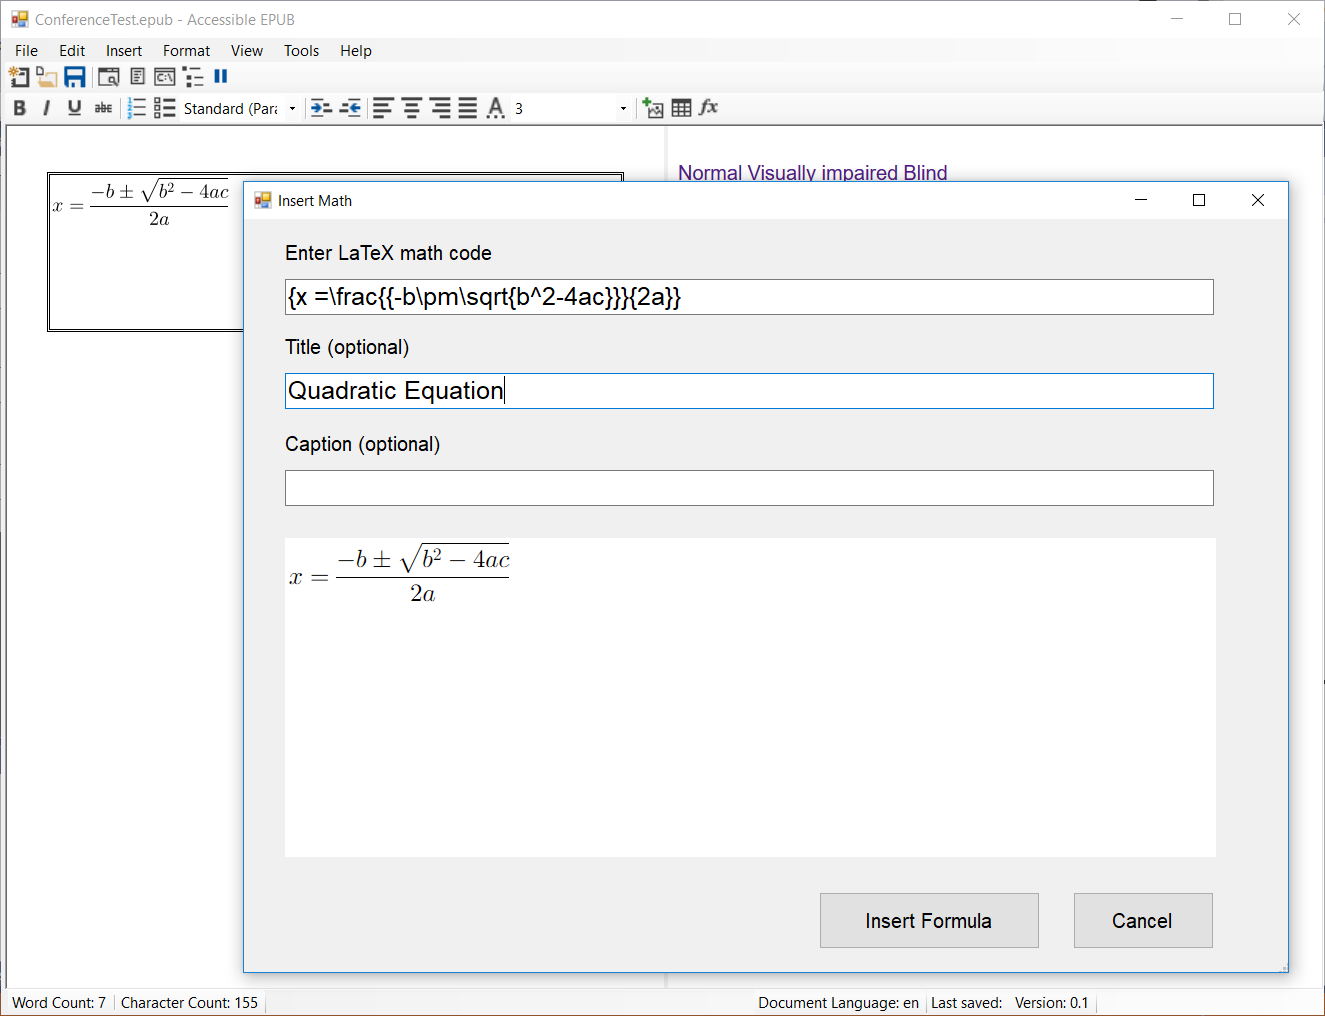
\includegraphics[width=\textwidth*4/5]{figures/AccessibleEPUBequationNew.PNG}
	\caption{Accessible EPUB equation editor}
	\label{fig:equationEditor}
\end{figure}

A focus of Accessible EPUB lies in the creation of documents for science, technology, engineering and mathematics (STEM) subjects and must therefore allow users to insert mathematical equations easily. The equation editor is shown in figure \ref{fig:equationEditor} and the user must enter LaTeX code, as it is simpler to write than MathML and several conversion programs exist. The input is then shown in equation form in the lower panel, without the user entering any additional command. This is done with the .NET library package, WpfMath\footnote{https://github.com/ForNeVeR/wpf-math}. It parses the LaTeX in real time and gives immediate feedback to the user. In its default implementation, an incorrect input results in a blank panel. This might be confusing to the user, as they might not know where exactly the error in the input lies. Fortunately, WpfMath contains the method \lstinline|HasError|, which detects if the input contains an error. This value was then passed to Accessible EPUB which then adds a red border around the panel, while leaving the parsed output of the last working input intact. The user is then able to get feedback to fix the issue while still having an idea where the problem was. 

However, WpfMath does not convert the LaTeX code to MathML. No .NET library was found which converts LaTeX to MathML is a satisfying manner. Consequently, external solutions had to found which follow the sequence of events.

\begin{enumerate}
	\item LaTeX code is passed on to an external program
	\item The external program converts the code to MathML
	\item MathML is passed back to Accessible EPUB which then inserts it into the EPUB.
\end{enumerate}

There were several factors which had to be considered when picking the external program. First of all, it had to be freely available, preferably open source, so that it can be distributed with Accessible EPUB. It should also require as few dependencies as possible. Lastly, it should not be a large program which would then greatly enlarge the file size. 

Some of the programs considered were LaTeXML\footnote{https://dlmf.nist.gov/LaTeXML/}, latex2mathml\footnote{https://github.com/Code-ReaQtor/latex2mathml} and TeX4ht\footnote{https://www.tug.org/tex4ht/} among others. Unfortunately, all of them have prerequisites, Perl, python and Tex, respectively. Finally, a program was found which satisfied the demands, pandoc\footnote{http://pandoc.org/}. It is not a very small program and with a size of 93.2 MB it does increase the size of the Accessible EPUB installation, but as pandoc can be run without dependencies this was deemed as an acceptable trade off.


%\textcolor{red}{pandoc } %┬▒}

\begin{figure}[h]
	\centering
	
\includegraphics[width=2em]{figures/pandocSigns.png}
	\caption{Signs shown instead of $\pm$ in pandoc}
	\label{fig:signsPlusMinus}
\end{figure}

However, there were still some issues with pandoc such as the plus-minus sign ($\pm$) not getting displayed properly when pandoc is run directly from Accessible EPUB. Instead of a plus-minus, the signs 
in figure \ref{fig:signsPlusMinus} are shown. This also happens if a formula with a plus-minus sign is given as input parameter and pandoc prints the results of the conversion in the command shell of windows. This is an issue with the encoding the command shell of Microsoft Windows uses. It cannot display some signs, such as even a simple minus sign (-). The conversion with pandoc also creates issues. The MathML specification \cite{mathMLrec} encodes several signs, including plus-minus. The encoded string is "\&PlusMinus;", which can be displayed in the command shell of windows. Pandoc does not use these encodings and uses the normal signs, which creates problems. The signs are shown normally if pandoc creates a stand alone HTML file with the \lstinline|-s| option which can be viewed individually, but not when only the relevant MathML part is created. The problem is further compounded that using the output option, \lstinline|-o|, of pandoc still produces the same encoding error. The signs are shown properly if the results are instead passed to a file with a redirect (">") in the command shell. This means that pandoc cannot be called directly from Accessible EPUB and instead the command shell program of Microsoft Windows, cmd.exe, has to be called as shown in figure \ref{fig:execPandoc}. \lstinline|accFile| refers to the file where the entered LaTeX code is saved to. It is then used here and the results, \lstinline|formulaResult| is inserted in the inner HTML code of the editor. \lstinline|CreateNoWindow| and \lstinline|WindowStyle| are used to not show a command shell popping up. It used to be only shown for a moment, but it might confuse the user.

\begin{figure}[h]
	
	\begin{lstlisting}
	var proc = new Process
	{
		StartInfo = new ProcessStartInfo
		{
			//FileName = "pandoc", //Path.Combine(pandoc, "pandoc"),
			FileName = @"c:\windows\system32\cmd.exe",
			Arguments = @"/c pandoc --mathml " + accFile + " > " + formulaResult,
			//UseShellExecute = false,
			//RedirectStandardOutput = false,
			CreateNoWindow = true,
			WindowStyle = ProcessWindowStyle.Hidden
		}
	}; 
	\end{lstlisting}
	\caption{The C\# code to execute pandoc}
	\label{fig:execPandoc}
\end{figure}

When the Accessible EPUB was installed on computers, there was another issue with pandoc. The file pandoc writes to the pandoc folder itself. While this worked before, it did not work when the editor was installed. The editor does not have permission to write to the pandoc folder, so it now writes to the folder for temporary files instead.

The MathML code from pandoc is then inserted in the inner HTML of the editor. However, Internet Explorer  cannot display MathML and the editor display it as shown in figure \ref{fig:IEmathml}. So a workaround had to be found. WpfMath can be used to create SVGs and PNGs of the mathematical formulas entered. So a SVG of the entered formula is generated and inserted into the editor with the MathML code. The CSS used by the editor hides the MathML and only shows the SVG. On the other hand, the preview browser hides the SVG and shows the MathML. The class \lstinline|toRemove| of the image in figure \ref{fig:mathSVG} is not shown in the EPUB, but the division tag of HTML, \lstinline|div|, with the class \lstinline|math| is shown. The SVG is also used as an alternative image if the EPUB reading system doesn't support MathML and supports the \lstinline|altimg| attribute,  as shown in the \lstinline|<math>| tag in figure \ref{fig:mathSVG}. 

\begin{figure}[h]
	
	\begin{lstlisting}
<FIGURE>
<IMG title="Quadratic Equation " class="toRemove" alt="{x=\frac{-b\pm\sqrt{b^2-4ac}}{2a}}" src="C:\Users\Sachin\AppData\Local\Temp\AccessibleEPUB\ConferenceTestJs\OEBPS\Images\Quadratic Equation.svg">

<DIV class="math" role="math">
<math title="Quadratic Equation" xmlns="http://www.w3.org/1998/Math/MathML" 
altimg="C:\Users\Sachin\AppData\Local\Temp\AccessibleEPUB\ConferenceTestJs\OEBPS\Images\Quadratic Equation.svg" 
alttext="{x=\frac{-b\pm\sqrt{b^2-4ac}}{2a}}">
...
<P class="transparent">${x=\frac{-b\pm\sqrt{b^2-4ac}}{2a}}$</P></FIGURE>

	\end{lstlisting}
\caption{The inner HTML of the editor showing how a SVG is shown instead of the MathML}
\label{fig:mathSVG}
\end{figure}

\subsection{EPUB work behind the scenes}

\begin{figure}[h]
	\centering
	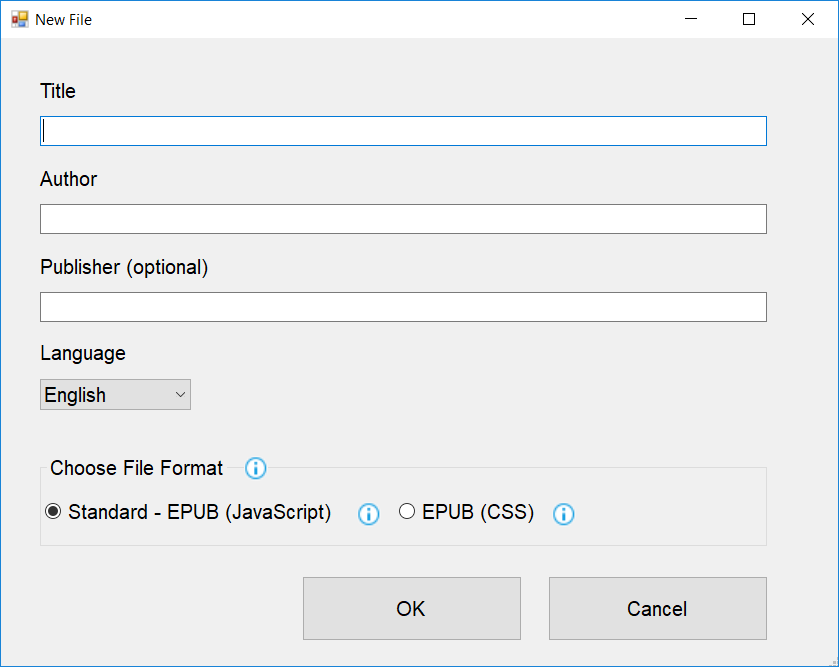
\includegraphics[width=\linewidth*4/5]{figures/newFileDialogBox.png}
	\caption{The dialog box shown when a new file is created}
	\label{fig:newFileDialogBox}
\end{figure}

While the content documents of an EPUB are the most important part, EPUBs require the package file referenced in chapter \ref{ch:Introduction} to be updated. The user should not have to do anything with the package file, named \lstinline|content.opf|. The first section \lstinline|metadata| is filled in when a new document is created and the new file dialog box is shown, as seen in \ref{fig:newFileDialogBox}. Accessible EPUB requires the title and author, while the EPUB specification does not require an author. In many EPUB reading systems the data used to identify a book normally consists of both the title and author so it is mandatory here. The publisher is not required, but will be useful to identify material from educational institutions. The only language choices currently available are English and German, but more languages will be added later in the development. 

The \lstinline|manifest| declaration contains all of the files in the EPUB document. Files not declared might not be shown properly. The user should not have anything to do with the manifest and it should be updated automatically. This is done when the user saves the file. The program looks through the whole folder and checks the file type and enter both it and the location into the manifest. An example is shown in figure \ref{fig:manifestExample}. The \lstinline|id| element is taken from the file name. Only the navigation documents have predefined ones. The \lstinline|href| element is the path from the package document. The \lstinline|media-type| is determined from the file type and the appropriate declaration found in the EPUB specification.

The \lstinline|spine| section is already predetermined. If support for multiple content files is added, then the ability to change the spine and by extension the reading order will be included in Accessible EPUB.

\begin{figure}[h]
	%	\centering
	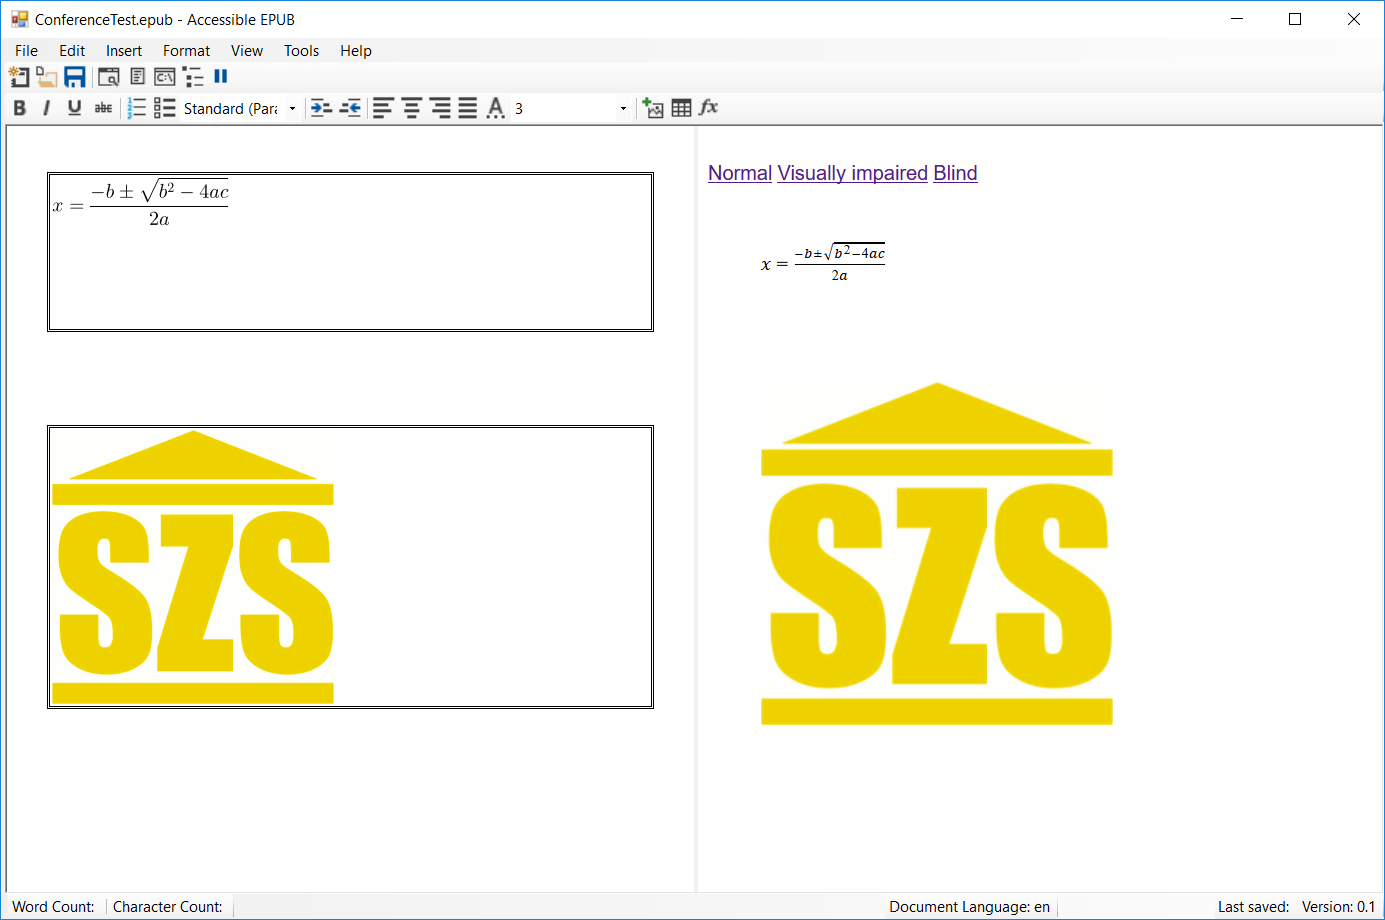
\includegraphics[width=\linewidth]{figures/AccessibleEPUBmathSZSvi.png}
	\begin{lstlisting}
	<manifest>
		<item id="Quadratic Equation.svg" href="Images/Quadratic Equation.svg" media-type="image/svg+xml"/>
		<item id="SZS.png" href="Images/SZS.png" media-type="image/png"/>
		<item id="style.css" href="Styles/style.css" media-type="text/css"/>
		<item id="Content.xhtml" href="Text/Content.xhtml" media-type="application/xhtml+xml"/>
		<item id="navid" href="Text/nav.xhtml" media-type="application/xhtml+xml" properties="nav"/>
		<item id="ncx" href="toc.ncx" media-type="application/x-dtbncx+xml"/>
	</manifest>
	\end{lstlisting}
	\caption{A sample EPUB of the CSS document standard and its corresponding manifest}	
	\label{fig:manifestExample}
\end{figure}

\subsubsection{Inserting images and tables}

\begin{figure}[h]
	\centering
	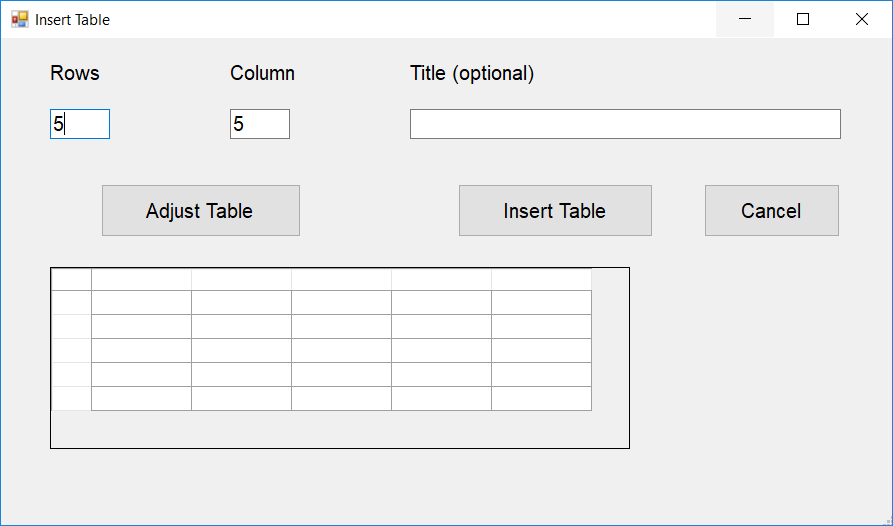
\includegraphics[width=\linewidth]{figures/TableDialogBox.png}
	\caption{The dialog box shown when the user wants to insert a table}
	\label{fig:tableDialogBox}
\end{figure}

Accessible EPUB allows the user to insert tables with the dialog box shown in figure \ref{fig:tableDialogBox}. The bottom half of the figure shows the C\# element, DataGridView. The size of it changes whenever the focus leaves the row or column text field by pressing the tab key or just presses elsewhere with the mouse. The user can also press the "Adjust Table" button. The alternative would have been to change the size whenever the values in the text fields are changed, but a useful feature is that values entered in the DataGridview are not lost if the size is increased or reduced. This allows for more flexibility in the table creation. 

\begin{figure}[h]
	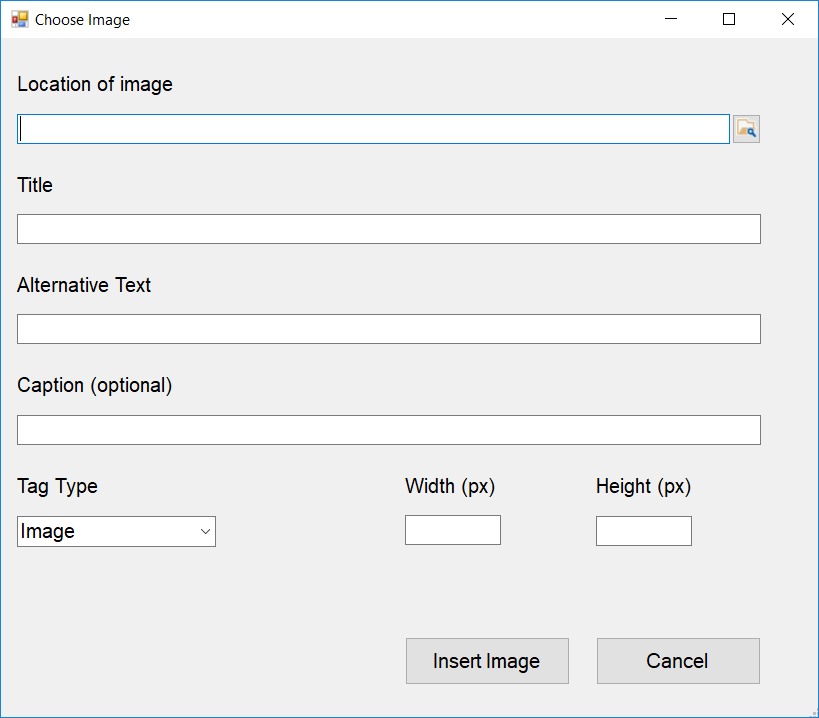
\includegraphics[width=\linewidth]{figures/imageDialogBox.png}	
	\caption{Insert image window of Accessible EPUB}
	\label{fig:imageDialogBox}
\end{figure}

The user is also able to add images with the window shown in figure \ref{fig:imageDialogBox}. The three mandatory elements are the location of the an image, a title and some alternative text. The title allows users with screen reader to identify the image and skip it if desired. Alternative text is also a must to maintain accessibility for all users. Captions are optional and are always inserted below the image. In future it is planned to allow users to add the caption above the image too. An important accessibility feature mentioned in \cite{augenbitWiki} is the use of image tag types. The choice of image tags automatically adjust to the current document language, irrespective of the program language. There are a few default tag types, but the user can type their own tag types in. In future the user will be able to add their own tags and save them so that they can be picked from the menu.

\begin{comment}
\textcolor{red}{An Thorsten: Das Einfügen der Bilder, Formeln und Tabellen hatten alle Probleme, somit werde diese drei definitiv erwähnen. Ich bin nicht sicher, ob ich alle Fenster auch diskutieren muss, da paar davon wenige Probleme hatten. Einstellungen und About waren relativ einfach und schmerzfrei, und deshalb kann ich nur kurz was dazu sagen. Was meinst du?}
\end{comment}
